\documentclass{sigchi}

% Use this section to set the ACM copyright statement (e.g. for
% preprints).  Consult the conference website for the camera-ready
% copyright statement.

% Copyright
% \CopyrightYear{2016}
%\setcopyright{acmcopyright}
% \setcopyright{acmlicensed}
%\setcopyright{rightsretained}
%\setcopyright{usgov}
%\setcopyright{usgovmixed}
%\setcopyright{cagov}
%\setcopyright{cagovmixed}
% DOI
% \doi{}
% ISBN
% \isbn{}
%Conference
% \conferenceinfo{}{}
%Price
% \acmPrice{}

% Load basic packages
\usepackage{balance}       % to better equalize the last page
\usepackage{graphics}      % for EPS, load graphicx instead 
\usepackage[T1]{fontenc}   % for umlauts and other diaeresis
\usepackage{txfonts}
\usepackage{mathptmx}
\usepackage[pdflang={en-US},pdftex]{hyperref}
\usepackage{color}
\usepackage{booktabs}
\usepackage{textcomp}


% Some optional stuff you might like/need.
\usepackage{microtype}        % Improved Tracking and Kerning
% \usepackage[all]{hypcap}    % Fixes bug in hyperref caption linking
\usepackage{ccicons}          % Cite your images correctly!
% \usepackage[utf8]{inputenc} % for a UTF8 editor only

% If you want to use todo notes, marginpars etc. during creation of
% your draft document, you have to enable the "chi_draft" option for
% the document class. To do this, change the very first line to:
% "\documentclass[chi_draft]{sigchi}". You can then place todo notes
% by using the "\todo{...}"  command. Make sure to disable the draft
% option again before submitting your final document.
\usepackage{todonotes}

% Paper metadata (use plain text, for PDF inclusion and later
% re-using, if desired).  Use \emtpyauthor when submitting for review
% so you remain anonymous.
\def\plaintitle{Maze Gaze - A Gaze-Based Multiplayer Game}
\def\plainauthor{Kevin Müller, Marco Siweris, Lena}
\def\emptyauthor{}
\def\plainkeywords{eye-tracking; gaze-based interaction; multi-user interaction; human computer interaction;}
\def\plaingeneralterms{Documentation, Standardization}

% llt: Define a global style for URLs, rather that the default one
\makeatletter
\def\url@leostyle{%
  \@ifundefined{selectfont}{
    \def\UrlFont{\sf}
  }{
    \def\UrlFont{\small\bf\ttfamily}
  }}
\makeatother
\urlstyle{leo}

% To make various LaTeX processors do the right thing with page size.
\def\pprw{8.5in}
\def\pprh{11in}
\special{papersize=\pprw,\pprh}
\setlength{\paperwidth}{\pprw}
\setlength{\paperheight}{\pprh}
\setlength{\pdfpagewidth}{\pprw}
\setlength{\pdfpageheight}{\pprh}

% Make sure hyperref comes last of your loaded packages, to give it a
% fighting chance of not being over-written, since its job is to
% redefine many LaTeX commands.
\definecolor{linkColor}{RGB}{6,125,233}
\hypersetup{%
  pdftitle={\plaintitle},
% Use \plainauthor for final version.
%  pdfauthor={\plainauthor},
  pdfauthor={\emptyauthor},
  pdfkeywords={\plainkeywords},
  pdfdisplaydoctitle=true, % For Accessibility
  bookmarksnumbered,
  pdfstartview={FitH},
  colorlinks,
  citecolor=black,
  filecolor=black,
  linkcolor=black,
  urlcolor=linkColor,
  breaklinks=true,
  hypertexnames=false
}

% create a shortcut to typeset table headings
% \newcommand\tabhead[1]{\small\textbf{#1}}

% End of preamble. Here it comes the document.
\begin{document}

\title{\plaintitle}

\numberofauthors{3}
\author{%
  \alignauthor{Kevin M{\"u}ller\\
    \affaddr{Saarland University}\\
    \affaddr{Saarbr{\"u}cken, Germany}\\
    \email{s9kvmuel@stud.uni-saarland.de}}\\
  \alignauthor{Marco Siveris\\
    \affaddr{Saarland University}\\
    \affaddr{Saarbr{\"u}cken, Germany}\\
    \email{e-mail address}}\\
  \alignauthor{Lena Hornberger\\
    \affaddr{Saarland University}\\
    \affaddr{Saarbr{\"u}cken, Germany}\\
    \email{e-mail address}}\\
}

\maketitle

\begin{abstract}
  UPDATED---\today.
\end{abstract}

% \keywords{\plainkeywords}

\section{Introduction}
% todo

\section{Graphics}
\begin{figure}
\centering
  
\includegraphics[width=0.9\columnwidth]{figures/sigchi-logo}
  \caption{Insert a caption below each figure. Do not alter the
    Caption style.  One-line captions should be centered; multi-line
    should be justified. }~\label{fig:figure1}
\end{figure}

\section{References and Citations}
Use a numbered list of references at the end of the article, ordered
alphabetically by last name of first author, and referenced by numbers
in
brackets~\cite{acm_categories,ethics,Klemmer:2002:WSC:503376.503378}.
Your references should be published materials accessible to the
public. Internal technical reports may be cited only if they are
easily accessible (i.e., you provide the address for obtaining the
report within your citation) and may be obtained by any reader for a
nominal fee. Proprietary information may not be cited. Private
communications should be acknowledged in the main text, not referenced
(e.g., ``[Borriello, personal communication]'').

References should be in ACM citation format:
\url{http://acm.org/publications/submissions/latex_style}. This
includes citations to internet
resources~\cite{acm_categories,cavender:writing,CHINOSAUR:venue,psy:gangnam}
according to ACM format, although it is often appropriate to include
URLs directly in the text, as above.

\begin{table}
  \centering
  \begin{tabular}{l r r r}
    % \toprule
    & & \multicolumn{2}{c}{\small{\textbf{Test Conditions}}} \\
    \cmidrule(r){3-4}
    {\small\textit{Name}}
    & {\small \textit{First}}
      & {\small \textit{Second}}
    & {\small \textit{Final}} \\
    \midrule
    Marsden & 223.0 & 44 & 432,321 \\
    Nass & 22.2 & 16 & 234,333 \\
    Borriello & 22.9 & 11 & 93,123 \\
    Karat & 34.9 & 2200 & 103,322 \\
    % \bottomrule
  \end{tabular}
  \caption{Table captions should be placed below the table. We
    recommend table lines be 1 point, 25\% black. Minimize use of
    table grid lines.}~\label{tab:table1}
\end{table}

\section{Figures/Captions}

Place figures and tables at the top or bottom of the appropriate
column or columns, on the same page as the relevant text (see
Figure~\ref{fig:figure1}). A figure or table may extend across both
columns to a maximum width of 17.78 cm (7 in.).

\begin{figure*}
  \centering
  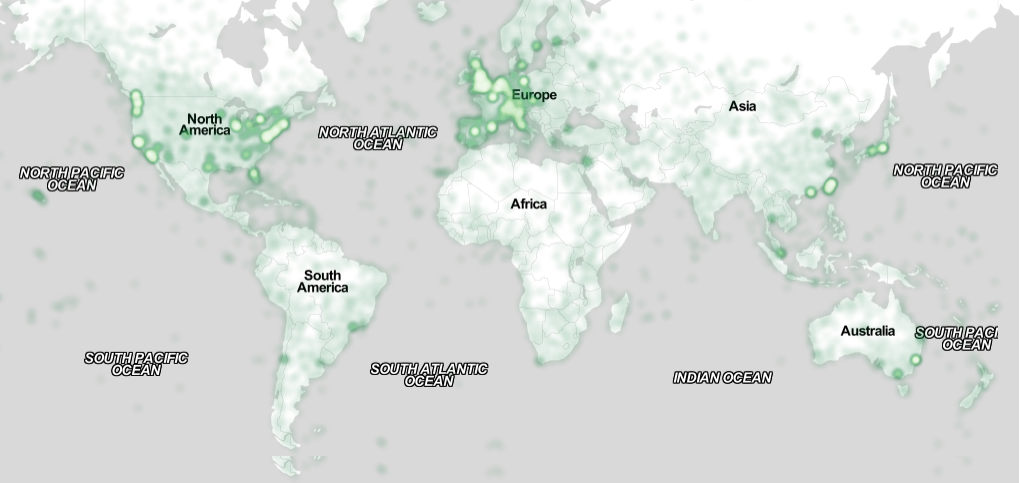
\includegraphics[width=1.75\columnwidth]{figures/map}
  \caption{In this image, the map maximizes use of space. You can make
    figures as wide as you need, up to a maximum of the full width of
    both columns. Note that \LaTeX\ tends to render large figures on a
    dedicated page. Image: \ccbynd~ayman on
    Flickr.}~\label{fig:figure2}
\end{figure*}


\section{Quotations}
Quotations may be italicized when \textit{``placed inline''} (Anab,
23F).

\begin{quote}
Longer quotes, when placed in their own paragraph, need not be
italicized or in quotation marks when indented (Ramon, 39M).  
\end{quote}

\section{Language, Style, and Content}

The written and spoken language of SIGCHI is English. Spelling and
punctuation may use any dialect of English (e.g., British, Canadian,
US, etc.) provided this is done consis- tently. Hyphenation is
optional. To ensure suitability for an international audience, please
pay attention to the following:

\begin{itemize}
\item Write in a straightforward style.
\item Try to avoid long or complex sentence structures.
\item Briefly define or explain all technical terms that may be
  unfamiliar to readers.
\item Explain all acronyms the first time they are used in your
  text---e.g., ``Digital Signal Processing (DSP)''.
\item Explain local references (e.g., not everyone knows all city
  names in a particular country).
\item Explain ``insider'' comments. Ensure that your whole audience
  understands any reference whose meaning you do not describe (e.g.,
  do not assume that everyone has used a Macintosh or a particular
  application).
\item Explain colloquial language and puns. Understanding phrases like
  ``red herring'' may require a local knowledge of English.  Humor and
  irony are difficult to translate.
\item Use unambiguous forms for culturally localized concepts, such as
  times, dates, currencies, and numbers (e.g., ``1--5--97'' or
  ``5/1/97'' may mean 5 January or 1 May, and ``seven o'clock'' may
  mean 7:00 am or 19:00). For currencies, indicate equivalences:
  ``Participants were paid {\fontfamily{txr}\selectfont \textwon}
  25,000, or roughly US \$22.''
\item Be careful with the use of gender-specific pronouns (he, she)
  and other gendered words (chairman, manpower, man-months). Use
  inclusive language that is gender-neutral (e.g., she or he, they,
  s/he, chair, staff, staff-hours, person-years). See the
  \textit{Guidelines for Bias-Free Writing} for further advice and
  examples regarding gender and other personal
  attributes~\cite{Schwartz:1995:GBF}. Be particularly aware of
  considerations around writing about people with disabilities.
\item If possible, use the full (extended) alphabetic character set
  for names of persons, institutions, and places (e.g.,
  Gr{\o}nb{\ae}k, Lafreni\'ere, S\'anchez, Nguy{\~{\^{e}}}n,
  Universit{\"a}t, Wei{\ss}enbach, Z{\"u}llighoven, \r{A}rhus, etc.).
  These characters are already included in most versions and variants
  of Times, Helvetica, and Arial fonts.
\end{itemize}


\balance{}


% REFERENCES FORMAT
% References must be the same font size as other body text.
\bibliographystyle{SIGCHI-Reference-Format}
\bibliography{sample}

\end{document}

%%% Local Variables:
%%% mode: latex
%%% TeX-master: t
%%% End:
